\newcommand{\drawsequence}[4]{%
  % #1: number of ticks
  % #2: comma-separated list of actions
  % #3: comma-separated list of probabilities
  % #4: total probability
  \begin{center}
    \begin{tikzpicture}[scale=0.8]
      % Draw the timeline
      \draw[->, thick] (0,0) -- (#1+0.65,0);
      
      % Draw tick marks
      \foreach \x in {1,...,#1} {
        \draw[thick] (\x,0.15) -- (\x,-0.15);
      }
      
      % Labels
      \node[left] at (0,1.) {\textbf{Action:}};
      \node[left] at (0,-1) {\textbf{Prob.:}};
      
      \foreach [count=\i] \action in {#2} {
        \node[minimum width=2.0cm, minimum height=0.8cm] at (\i,1.) {\action};
      }
      
      % Process the probabilities
      \foreach [count=\i] \prob in {#3} {
        \node at (\i,-1.) {\prob};
      }
      
      % Add total probability at the end
      \node at (#1+0.75,-1.) {$=$};
      \node at (#1+1.5,-1.) {#4};
    \end{tikzpicture}
  \end{center}
}

\section{Refulgent Arrow}

In addition to procs from Repertoire, most of Bard's GCDs, Burst Shot, Iron Jaws, Stormbite, and Caustic Bite, have a 35\% chance of granting Hawk's Eye, allowing for the execution of Refulgent Arrow (RA). Note however, that RA cannot grant Hawk's Eye. These actions are referred to as Hawk's Eye granting actions (HA). For a sequence of $n$ GCDs consisting of HA + RA, $k_{ra}$ of them can consist of RA and the corresponding damage distribution will be a mixture distribution,

\begin{equation}
  P(D) = \sum_{k_{ra}} w(k_{ra}) P(D_{ra}; k) \ast P(D_{ha}; n - k).
  \label{eqn:ra_mixture}
\end{equation}

The weights in eqn. \ref{eqn:ra_mixture} are equal to the probability distribution of RA procs, $P_{ra}(k_{ra}; n, p_{ra})$.\footnote{If $n$ is randomly distributed due to Army's Paeon, one could construct a joint probability distribution and average over all possible combinations.} This distribution somewhat resembles a binomial distribution, but is constrained such that a success (RA) is always succeeded by a failure (HA). A GCD sequence will be a set of non-independent trials, $\{ x_i \}$, where the probability for trial $i$ is

\begin{equation}
  P(x_i) = 
    \begin{cases}
       p & i = 1 \text{ or } x_{i-1} = \textrm{RA} \\
        0 & x_{i-1} = \textrm{HA}
    \end{cases}
    \label{eqn:ra_bernoulli}
\end{equation}

Intuitively, eqn. \ref{eqn:ra_bernoulli} simply forbids two RAs in a row; the rest of the derivation follows by counting valid patterns. Deriving the probability distribution for a sequence of trials is similar to deriving the binomial distribution from a sequence of Bernoulli trials: enumerate the sample space and find the probability of each sample point. As a motivating example, consider a $n=5$ GCD sequence consisting of $n-k_{ra} = 2$ HA and $k_{ra} = 3$ RA. One valid sample point of HA and RA usages is

\drawsequence{5}{HA, HA, RA, HA, HA}{65\%, 65\%, 35\%, 100\%, 65\%}{10\%}

Because of the non-consecutive RA constraint, a sample point with $n$ actions has at most $\lfloor \frac{n +1}{2} \rfloor$ RA successes, bounding $k_{ra}$ to $k_{ra} \in \{0, 1, 2, \dots, \lfloor \frac{n +1}{2} \rfloor \}$. For a sample point of $n$ actions, the number of ways to arrange with $k_{ra}$ RA successes, with no RA successes adjacent to each other is

\begin{equation}
    a(k_{ra}; n) = \binom{n-k_{ra}+1}{k_{ra}}
    \label{eqn:ra_sequences_a}
\end{equation}

This resembles the binomial coefficient, but with different arguments to account for the constraints from eqn. \ref{eqn:ra_bernoulli}. The probability of each sample point is also non-uniform because a HA following an RA is 100\%. For example, any sample point that does not end with RA

\drawsequence{3}{RA, HA, HA}{35\%, 100\%, 65\%}{23\%}

will have a different probability than a sample point that does end with RA,

\drawsequence{3}{HA, HA, RA}{65\%, 65\%, 35\%}{15\%}

In general, a sample point ending with on RA will not have a guaranteed HA, meaning there are $n-2k_{ra}+1$ HA which occur with probability $(1-p_{ra})$. Sample points ending with HA will have all possible guaranteed HA actions, $n-2k_{ra}$. The probability of a particular sample point is

\begin{equation}
p_{ra}^{k_{ra}}
    \begin{cases}
        (1-p_{ra})^{n-2k_{ra}} & \text{if last action is HA} \\
        (1-p_{ra})^{n-2k_{ra}+1} & \text{if last action is RA}
    \end{cases}
\end{equation}

The number of each type of sample points must be counted so the probability distribution is properly weighted and normalized. For a given $k_{ra}$, the number of sample points which end in RA, $a_{ra}(k_{ra}; n)$ is

\begin{equation}
    a_{ra}(k_{ra}; n) = \binom{n - k_{ra}}{k_{ra} - 1}
    \label{eqn:ra_sequences_a_ra_end}
\end{equation}

The number of sample points ending in HA, $a_{ha}(k_{ra}; n) = a(k_{ra}; n) - a_{ra}(k_{ra}; n)$, can be expressed using eqn. \ref{eqn:ra_sequences_a} and eqn. \ref{eqn:ra_sequences_a_ra_end}, 

\begin{equation}
a_{ha}(k_{ra}; n) = \binom{n-k_{ra}+1}{k_{ra}} - \binom{n - k_{ra}}{k_{ra} - 1}
\end{equation}

For a sequence containing $n$ HA and RA trials, the probability that $k_{ra}$ HA are granted is

\begin{equation}
    \begin{split}
        P_{ra}(k_{ra}; n, p_{ra}) &= a_{ha}(k_{ra}; n) p_{ra}^{k_{ra}} (1 - p_{ra})^{n-2k_{ra}} \\ 
        &+ a_{ra}(k_{ra}; n) p_{ra}^{k_{ra}} (1 - p_{ra})^{n - 2k_{ra} + 1}
    \end{split}
    \label{eqn:p_ra_ind}
\end{equation}

An example of the RA proc distribution is shown for $n=10$ and $n=50$, Figure \ref{fig:ra-proc-distribution}. Like the binomial distribution, the RA proc distribution also approaches a normal distribution as $n$ grows large.

\begin{figure}[H]
  \centering
  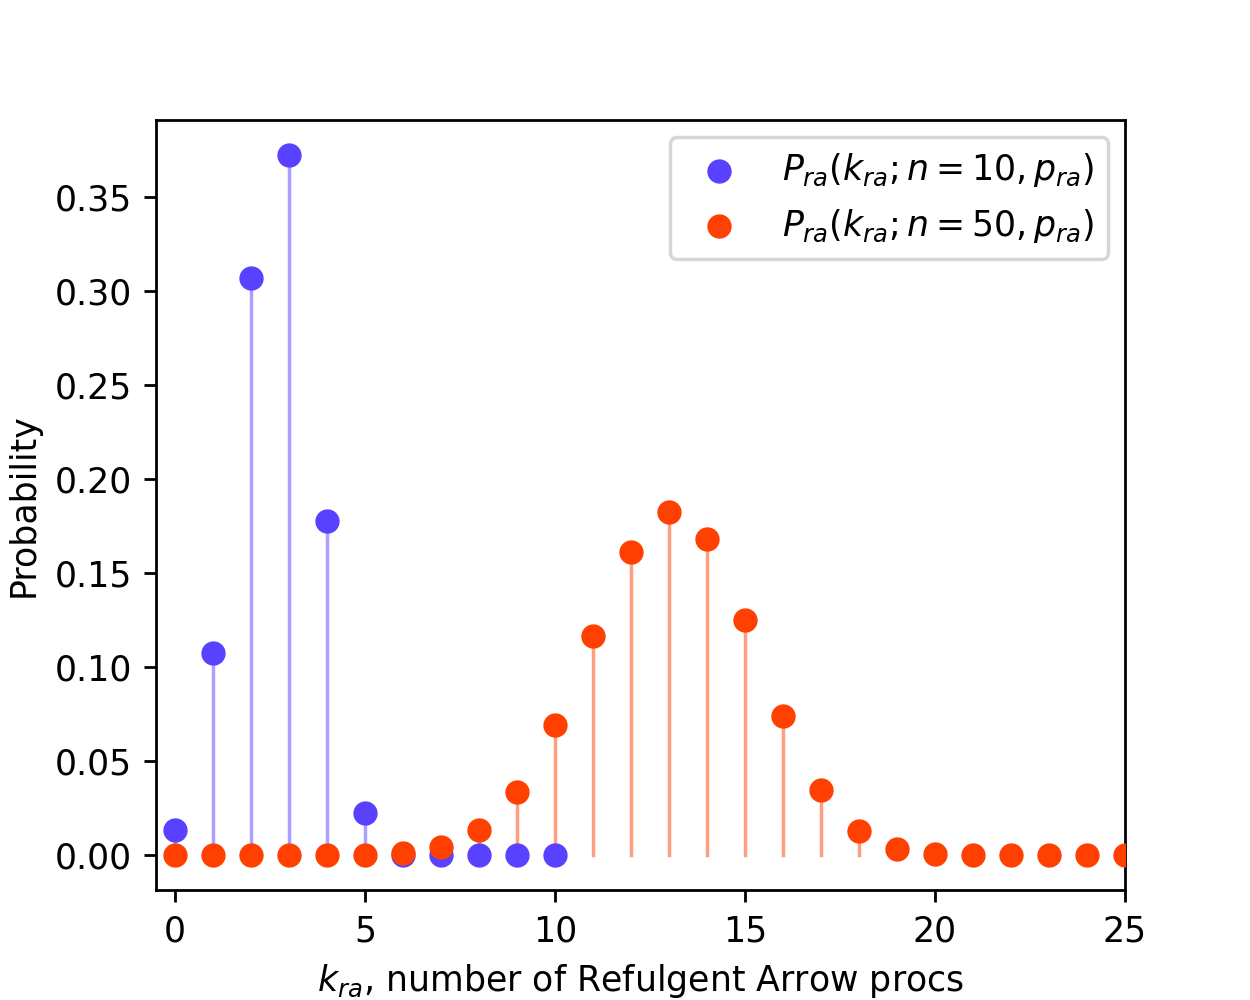
\includegraphics[scale=0.65]{img/ra-proc-distribution.png}
  \caption{Refulgent Arrow proc distribution for $n=10$ and $n=50$. Note the number of HA procs is $n-k_{ra}$.}
  \label{fig:ra-proc-distribution}
\end{figure}

Eqn. \ref{eqn:p_ra_ind} can be further analyzed and compared to binomial distribution\footnote{Recall that the binomial distribution has a mean of $np$ and variance of $np(1-p)$.} by computing the mean from the first moment of the PMF (for conciseness, subscripts are dropped),

\begin{equation}
  \begin{split}
  \mu &= E[X] = \frac{np}{1+p} + \frac{p^2}{(1+p)^2}(1 - (-p)^n) \\
      &\approx \frac{np}{1+p}
  \end{split}
  \label{eqn:mean_ra}
\end{equation}

The variance can be also computed from the first and second moment

\begin{equation}
  \begin{split}
  \sigma^2 &= E[X^2] - E[X]^2 \\
  &= \frac{np(1-p)}{(1+p)^2} + \frac{2p^3}{(1+p)^3}\frac{1-(-p)^n}{1+p} \\
  &- \frac{p^4}{(1+p)^4}(1-(-p)^n)^2 - \frac{p^2}{(1+p)^2}(-p)^n \\
  &\approx \frac{np(1-p)}{(1+p)^2}
  \end{split}
  \label{eqn:var_ra}
\end{equation}

Both eqn. \ref{eqn:mean_ra} and eqn. \ref{eqn:var_ra} have transient probability ratios, which are $< 1$. As $n$ grows large, these terms will be negligible and can be omitted. When these extra terms are dropped, the mean and variance closely resemble the mean and variance binomial distribution, respectively. Note that both eqn. \ref{eqn:p_ra_ind} and eqn. \ref{eqn:var_ra} will always be smaller than the mean and variance of a binomial distribution, respectively, as $(1+p) > 1$. This intuitively makes sense, as the total number of possible successes is restricted and always smaller than a binomial distribution.

Since $p_r = 0.35$, approximately 26\% of all HA / RA actions will be RA. One standard deviation is also $\approx 0.35 n^{1/2}$. For a sequence of 100 actions, there would be on average 26 RA procs with a standard deviation of $\pm3.5$ RA procs. The current potency difference between Refulgent Arrow and Burst Shot is 60 potency. At $n=100$ the probability distribution is roughly normal, so 68\% of runs would vary by up to $7 \times 60 = 420$ potency from Refulgent Arrow procs alone, ca. 2 Burst Shot usages.

One final consideration is that sequence of HA / RA usages is independent of buffs coming online and going offline. Conversely, the underlying damage distributions are dependent on what buffs are present. For example, consider a sequence of 36 HA / RA used across during Mage's Ballad and Army's Paeon. There is a single sequence for computing RA procs. The HA / RA will sample different one-hit distributions depending on the active song, so computing damage distributions requires partitioning the HA / RA sequence into separate sub-sequences and computing damage distributions separately. 


However, sub-sequences are not strictly independent. The current sub-sequence is coupled to the previous sub-sequence through whether it ends on RA, which forces a guaranteed HA. For example, if one subsequence ends with RA, the next subsequence must start with HA (100\% probability): $[\ldots, \text{RA}] | [\text{HA (100\%)}, \ldots]$. But if the previous subsequence ends with HA, the next can start with either HA (65\% probability) or RA (35\% probability). This short-lived memory also means these boundary effects will be quite small for large $n$. Under the assumption of well-aligned party buffs, the number of small $n$ valued sub-sequences is mainly limited to the opener and number of occurrences will be small compared to the total sub-sequences and their respective $n$ values. When modeling damage distributions, it is reasonable to treat sub-sequences as independent, especially since most typical combat scenarios result in sub-sequences with large $n$.

\subsection{Example calculation}

Here, it is shown how the damage distribution of HA / RA can be calculated for the duration The Wanderer's Minuet. This example highlights how to account for variable buff effects from Raging Strikes, Radiant Finale, and Battle Voice by partitioning the HA / RA sequence into sub-sequences by buffs and analyzing each sub-sequence separately. Table \ref{t:ra_rotation} depicts a simple rotation along with the corresponding sub-sequences of HA / RA.

\begin{table}[H]
\centering
\caption{Tabular depiction of various HA / RA sub-sequences during The Wanderer's Minuet.}

\begin{tabular}{@{}llcl@{}}
\toprule
GCD & Action  & Sub-seq. length  & Buffs                       \\ \midrule
0   & S. Bite &                    & \bufficons{wm} \\ 
1   & C. Bite &                    & \bufficons{wm} \\ \midrule
2   & HA / RA & 1                  & \bufficons{wm,bv} \\ \midrule
3   & HA / RA & \multirow{9}{*}{4} & \bufficons{wm,bv,rf,rs} \\
4   & -       &                    & \bufficons{wm,bv,rf,rs} \\
5   & -       &                    & \bufficons{wm,bv,rf,rs} \\
6   & -       &                    & \bufficons{wm,bv,rf,rs} \\
7   & HA / RA &                    & \bufficons{wm,bv,rf,rs} \\
8   & HA / RA &                    & \bufficons{wm,bv,rf,rs} \\
9   & HA / RA &                    & \bufficons{wm,bv,rf,rs} \\ \midrule
10  & HA / RA & 1                  & \bufficons{wm,rf,rs} \\ \midrule
11  & HA / RA & \multirow{11}{*}{8} & \bufficons{wm} \\
12  & HA / RA &                    & \bufficons{wm} \\
13  & HA / RA &                    & \bufficons{wm} \\
14  & HA / RA &                    & \bufficons{wm} \\
15  & HA / RA &                    & \bufficons{wm} \\
16  & HA / RA &                    & \bufficons{wm} \\
17  & HA / RA &                    & \bufficons{wm} \\
18  & HA / RA &                    & \bufficons{wm} \\ \bottomrule
\end{tabular}

\vspace{3pt}

\begin{tablenotes}%[para,flushleft]
\small
\item Buff legend: 

\includegraphics[height=1.1em]{img/icons/wm.png} = The Wanderer's Minuet;

\includegraphics[height=1.1em]{img/icons/bv.png} = Battle Voice;\\

\includegraphics[height=1.1em]{img/icons/rf.png} = Radiant Finale;

\includegraphics[height=1.1em]{img/icons/rs.png} = Raging Strikes.
\item Horizontal lines group HA / RA sub-sequences by buffs.
\item Records with `-' note non-HA / RA GCDs, which are omitted in this example calculation. This includes the guaranteed RA from Barrage.
\end{tablenotes}
\label{t:ra_rotation}
\end{table}


Note that although Resonant Arrow and Radiant Encore are also GCDs, they do not interact with granting Hawk's Eye and can be ignored in the HA / RA sequence. The following assumptions are also made:

\begin{itemize}
  \item A potential RA proc from the initial Stormbite usage is ignored, as this is recommended gameplay.
  \item The player is assumed to refresh DoTs with Iron Jaws one GCD earlier than needed, to avoid a situation where using an RA proc would lead to letting DoT effects fall off or an RA proc could be overwritten.
  \item For simplicity, the only HA analyzed will be Burst Shot, in lieu of the Iron Jaws present at the 8th or 9th GCD.
  \item The effect of Barrage granting an RA proc is omitted.
\end{itemize}

For comparison, the damage distribution is also sampled (which assumes no sub-sequence independence and is exact), and the damage distribution using the mode of RA procs from each sub-sequence is also computed. Figure \ref{fig:ra-dmg-distribution} shows these damage distributions.

\begin{figure}[H]
  \centering
  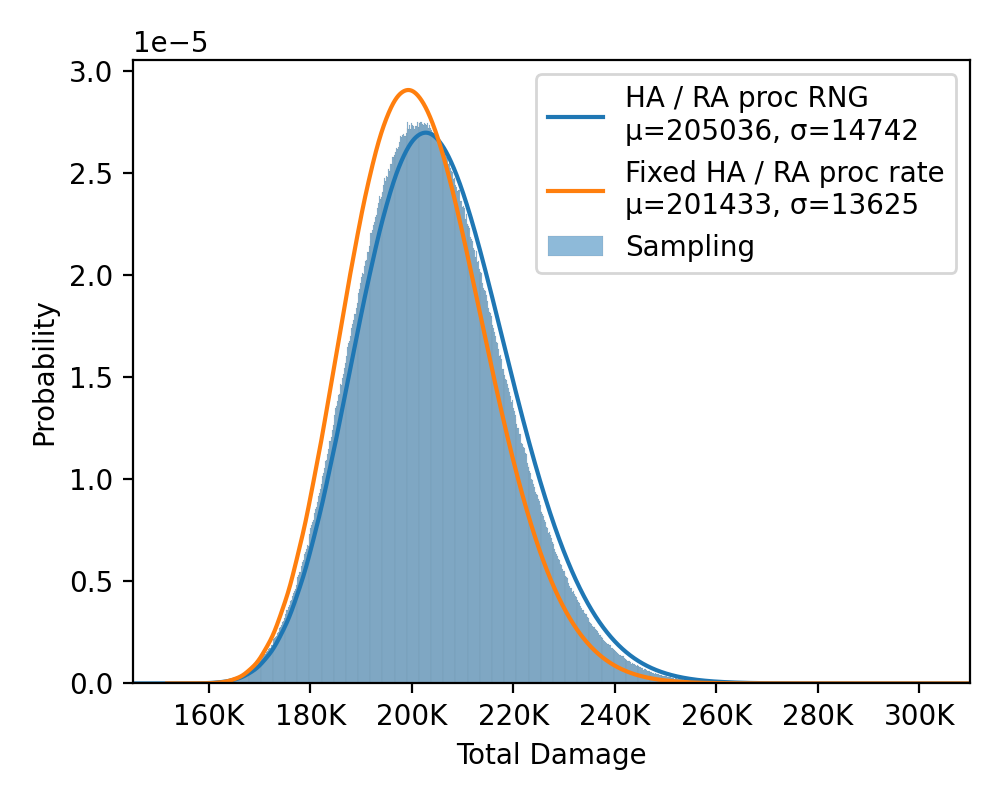
\includegraphics[scale=0.65]{img/ra-dmg-distribution.png}
  \caption{HA / RA damage distribution for eqn. \ref{eqn:ra_mixture} accounting for proc variability (blue line), exact sampling damage variability and proc variability (blue histogram), and assuming the average RA proc rate (orange). Sampling used 1,000 RA proc sample sequences, and each set of actions were sampled 10,000 times for damage variability.}
  \label{fig:ra-dmg-distribution}
\end{figure}

Comparing eqn. \ref{eqn:ra_mixture} and assuming sub-sequence independence, the two distributions match almost perfectly, as assuming sub-sequence independence is an excellent approximation. The damage distribution of each sub-sequence is shown in Appendix \ref{fig:app_ra_subseq}, and where it can be seen that the very small discrepancies are indeed due to the sequences of $n=1$. Compared to assuming an average RA proc rate, the mean is noticeably lower by ca. 5,000 damage. This is likely because all sub-sequences had their average rounded down to the nearest integer, resulting in lower damage across all sub-sequences. The standard deviation increases by about 8\% when fully accounting for RA procs for this 15 GCD sequence. Note however, that the DPS variance will decrease by $n^{-1/2}$, so for a full-length fight, the effects of RA proc variability will likely be even smaller.



